\documentclass{article}
\usepackage[utf8]{inputenc}
\usepackage[T1]{fontenc}
\usepackage{polski}
\usepackage{indentfirst}
\usepackage{lastpage}
\usepackage{graphicx} 
\graphicspath{ {./images/} }

\usepackage[section]{placeins}
\usepackage{fancyhdr}
\pagestyle{fancy}
\fancyhf{}
\lhead{Specyfikacja Funkcjonalna}
\rfoot{Strona \thepage \hspace{1pt} z \pageref{LastPage}}
\lhead{Spis treści}
\title{Specyfikacja Funkcjonalna dla projektu pt. \\ ,,Karetki w pogotowiu''}
\author{}
\date{}

\begin{document}
\maketitle

\begin{flushright}
\par ...
\vfill
\par
Wykonali:
\\Karolina Czachorska
\\Adrian Milewski
\\Maxymilian Kowalski
\\Bartłomiej Anczok
\\Data: 04.12.2020
\end{flushright}

\thispagestyle{empty}
\newpage
\begin{frame}{}
    \tableofcontents
\end{frame}
\newpage
\section{Opis teoretyczny}
\lhead{Projekt pt. "\textit{Karetki w pogotowiu}"}
{\fontsize{14}{14}\selectfont
Karetki w pogotowiu - 
jest to program mający na celu pomóc zespołowi ratowników z Karetek Pogotowia (KP) w jaki sposób przewozić pacjentów (P) do Ośrodków Medycznych (OM). Karetki przewożą pacjentów do najbliższego szpitala, obok którego znajduje się pacjent.
Jeśli okazuje się, że nie ma wolnych miejsc, jedzie do kolejnego najbliższego szpitala. W momencie gdy odwiedzimy wszystkie i w żadnym nie będzie miejsca, zostawiamy pacjenta.
\newline}
\section{Sposób wywołania programu}
{\fontsize{14}{14}\selectfont 

Aby skompilować i uruchomić program należy wejść do folderu z projektem i w terminalu wywołać komendę:
\\Windows:\\
\textbf{gradlew run}
\newline
\\Linux:\\
\textbf{./gradlew run}
\newline
}

\section{Dane wejściowe}
{\fontsize{14}{14}\selectfont 
Użytkownik będzie mógł przekazać plik do programu (za pomocą przycisku), w którym będą znajdować się:
\begin{itemize}
    \item Szpitale (id | nazwa | wsp. x | wsp. y | Liczba łóżek | Liczba wolnych łóżek)
    \item Obiekty (id | nazwa | wsp. x | wsp. y)
    \item Drogi (id | id\_szpitala | id\_szpitala | odległość)
\end{itemize}
\pagebreak
\textbf{Przykładowe dane w pliku:}
\newline
\newline
{\fontsize{10}{10}\selectfont 
\texttt{
\# Szpitale (id | nazwa | wsp. x | wsp. y | Liczba łóżek | Liczba wolnych łóżek)\\
1 | Szpital Wojewódzki nr 997 | 10 | 10 | 1000 | 100 \\
2 | Krakowski Szpital Kliniczny | 100 | 120 | 999 | 99\\
3 | Pierwszy Szpital im. Prezesa RP | 120 | 130 | 99 | 0\\
4 | Drugi Szpital im. Naczelnika RP | 10 | 140 | 70 | 1\\
5 | Trzeci Szpital im. Króla RP | 140 | 10 | 996 | 0\\
\\
\# Obiekty (id | nazwa | wsp. x | wsp. y)\\
1 | Pomnik Wikipedii | -1 | 50\\
2 | Pomnik Fryderyka Chopina | 110 | 55\\
3 | Pomnik Anonimowego Przechodnia | 40 | 70\\
\\
\# Drogi (id | id\_szpitala | id\_szpitala | odległość) \\
1 | 1 | 2 | 700\\
2 | 1 | 4 | 550\\
3 | 1 | 5 | 800\\
4 | 2 | 3 | 300\\
5 | 2 | 4 | 550\\
6 | 3 | 5 | 600\\
7 | 4 | 5 | 750\\
}
}
\newline
Występują również dwa sposoby na wczytanie danych o pacjentach:
\begin{itemize}
    \item Wciśnięcie odpowiedniego przycisku i wczytanie danych z pliku
    \item Podwójne kliknięcie na mapie, aby dodać pacjenta w danym miejscu
    \newline
    \newline
\end{itemize}

\textbf{Przykładowe dane w pliku z pacjentami:}
\newline
\newline
{\fontsize{10}{10}\selectfont 
\texttt{
\# Pacjenci (id | wsp. x | wsp.y)\\
1 | 20 | 20\\
2 | 99 | 105\\
3 | 23 | 40\\
}
}
}
\section{Dane wyjściowe}
{\fontsize{14}{14}\selectfont 
Po wczytaniu danych i wystartowaniu programu, ukaże nam się animacja przewozu pacjentów do szpitali. W przypadku, gdy danych jest zbyt dużo, aby wyświetlić animacje, pojawi się okno dialogowe z wypisywanymi po kolei opisami wydarzeń. 
Zostanie utworzony również plik wyjściowy w katalogu roboczym, zawierający po kolei opisane wydarzenia 
\newline}

\section{Działanie programu}
\subsection{Scenariusz ogólny}
{\fontsize{14}{14}\selectfont 
Użytkownik podaje dane w wyżej wymieniony sposób. W przypadku podania złych danych wyświetli się stosowny komunikat o napotkanym błędzie.
\newline 
W przypadku podania prawidłowych danych wejściowych program wykona obliczenia, wyświetli rezultaty oraz zakończy pracę. 
\newline}

\subsection{Scenariusz szczegółowy}
{\fontsize{14}{14}\selectfont 
Po uruchomianiu programu użytkownik ma dwie opcje: start oraz exit. W przypadku wybrania drugiej opcji, program kończy swoje działanie, natomiast jeżeli użytkownik wybierze opcję „start”, program przechodzi do następnego okna, w którym użytkownik ma możliwość wczytania odpowiednich plików.
\newline 
Użytkownik wczytuje plik z mapą. W momencie, gdy format pliku jest nieprawidłowy, np. ma za mało znaków dzielących, powtórzone ID lub nazwę szpitala/obiektu, błędne współrzędne itd. program przerywa wczytywanie pliku oraz zwraca informację na temat miejsca wystąpienia błędu oraz jego rodzaju. Następnie użytkownik wczytuje do programu pacjentów, może to zrobić na dwa sposoby. Pierwszym z nich jest podwójne kliknięcie na mapę natomiast drugim, jest wczytanie ich z pliku. W tym przypadku następuje weryfikacja poprawności wczytywanych danych. Jeżeli program wykryje błąd w pliku z pacjentami, podobnie jak w poprzednim przypadku, przerywa operację wczytywania danych oraz zwraca stosowany komunikat. 
\newline
Jeżeli udało się poprawnie wczytać dane o pacjentach oraz mapę, użytkownik może wybrać sposób wyświetlania informacji na temat przewozu pacjentów. Do wyboru ma opcję animacji graficznej oraz opcję przedstawienia tych informacji za pomocą logów. Po wybraniu jednej z opcji oraz kliknięciu start, program rozpoczyna swoje działanie. Po zakończeniu wszystkich operacji, niezależnie od wybranej opcji wyświetlenia informacji w GUI, program tworzy plik wyjściowy „output.txt” zawierający tekstowe przedstawienie transportu pacjentów w formie logów. 
\newline }
\pagebreak

\subsection{Ekrany działania programu}
{\fontsize{14}{14}\selectfont 
\begin{figure}[!h]
    \centering
    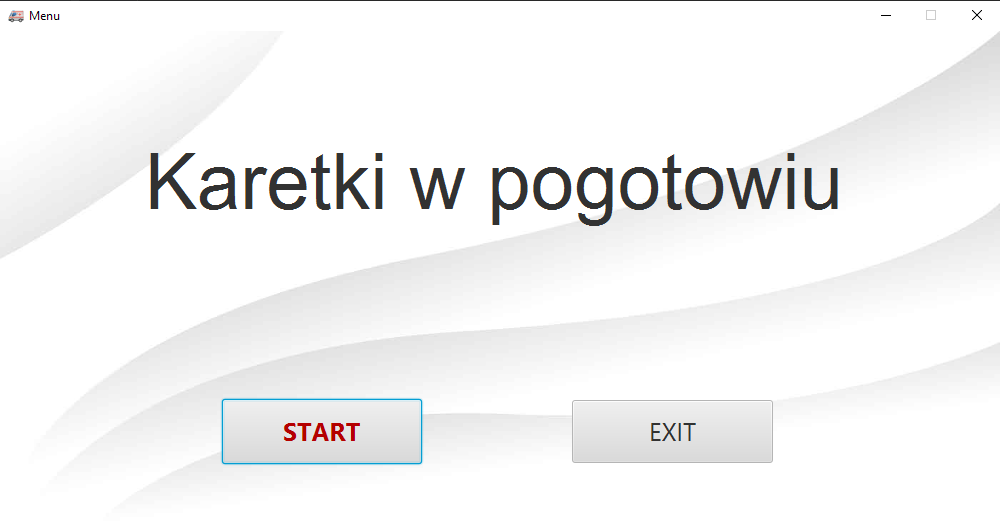
\includegraphics[width=1\textwidth]{images/ekran_startowy.png}
    \caption{Ekran startowy}
    
    \vspace*{\floatsep}
    
    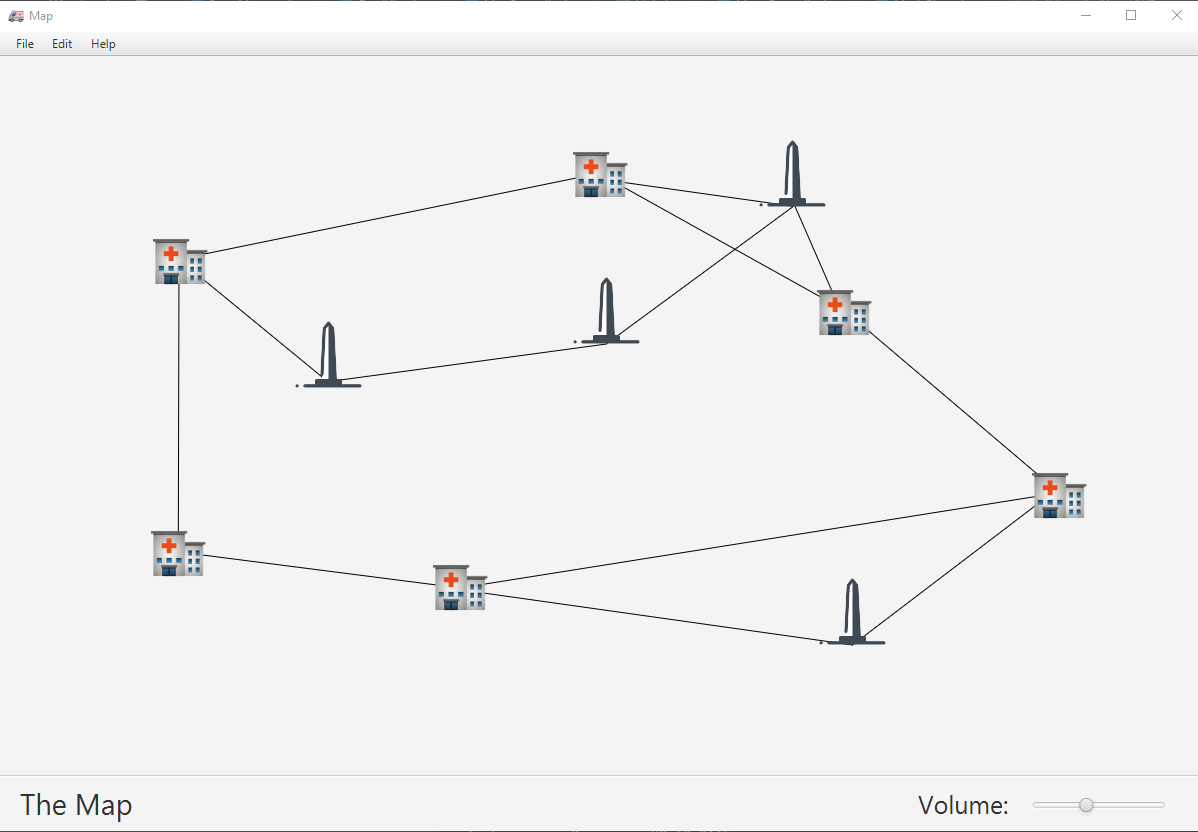
\includegraphics[width=1\textwidth]{images/przykladowa_mapa.png}
    \caption{Przykładowa mapa}
\end{figure}

\newline}

\section{Komunikaty o błędach}
{\fontsize{14}{14}\selectfont 
Program będzie odpowiednio zabezpieczony w stosunku do wszelkich nieprawidłowych działań podjętych przez użytkownika. Jeżeli wystąpi pewna nieprawidłowość, będą wyświetlane komunikaty w graficznym interfejsie użytkownika z dokładnym opisem błędu jaki został napotkany. Wszelkie niestosowne akcje, które będzie można napodkać w programie, przedstawione są w rozdziale "sytuacje wyjątkowe".
}

\section{Sytuacje wyjątkowe}
\begin{table}[!h]
    \centering
    \begin{tabular}{|p{6cm}|p{6cm}|}
        \hline
         Sytuacja wyjątkowa & Reakcja programu \\ \hline
         Wybór nieprawidłowego formatu pliku w oknie wybierania mapy bądź pacjentów & Program przerywa wczytywanie pliku i wyświetla komunikat o błędnym pliku wejściowym \\ \hline
         Nieodpowiedni typ danych jakiejkolwiek kolumny w pliku wejściowym & Program przerywa wczytywanie pliku i wyświetla komunikat: \emph{Zły typ danych w pliku wejściowym w wierszu <numer\_wiersza>} \\ \hline
         Nieodpowiednia liczba kolumn w wierszu & Program przerywa wczytywanie pliku i wyświetla komunikat: \emph{Nieodpowiednia liczba kolumn w pliku wejściowym w wierszu <numer\_wiersza>} \\ \hline
         Plik jest pusty & Program przerywa wczytywanie pliku i wyświetla komunikat: \emph{Plik nie może być pusty} \\ \hline
         Plik z mapą zawiera mniej niż trzy nagłówki & Program przerywa wczytywanie pliku i wyświetla komunikat: \emph{Plik powinien składać się z trzech części oddzielonych nagłówkami} \\ \hline
         Powtórzenie identyfikatora drogi lub pacjenta & Program przerywa wczytywanie pliku i wyświetla komunikat: \emph{Identyfikatory muszą być uniklane. Błąd w pliku wejściowym w wierszu <numer\_wiersza>} \\ \hline
         Liczba szpitali przekroczy 1000 & Program przerywa wczytywanie pliku i wyświetla komunikat: \emph{Liczba szpitali nie może przekraczać 1000} \\ \hline
         Próba dodania pacjenta poza mapą & Program przerywa dodawanie pacjenta i wyświetla komunikat: \emph{Pacjent musi się znajdować w obrębie mapy} \\ \hline
    \end{tabular}
\end{table}

\section{Testowanie programu}
{\fontsize{14}{14}\selectfont
W celu minimalizacji błędów oraz ułatwienia dalszej implementacji, do najważniejszych modułów w projekcie zostaną napisane testy sprawdzające poprawność działania poszczególnych funkcjonalności.
Testy będą niezależne od działania innych modółów w programie.}
\end{document}